%----------------------------------------------------------------
%
%  File    :  thesis.tex
%
%  Authors :  Keith Andrews, IICM, TU Graz, Austria
%             Manuel Koschuch, FH Campus Wien, Austria
%			  Sebastian Ukleja, FH Campus Wien, Austria
% 
%  Created :  22 Feb 96
% 
%  Changed :  14 Oct 2020
%
%  For suggestions and remarks write to: sebastian.ukleja@fh-campuswien.ac.at
% 
%----------------------------------------------------------------

% --- Setup for the document ------------------------------------

%Class for a book like style:
\documentclass[11pt,a4paper,oneside]{scrbook}
%For a more paper like style use this class instead:
%\documentclass[11pt,a4paper,oneside]{thesis}

%input encoding for windows in utf-8 needed for Ä,Ö,Ü etc..:
\usepackage[utf8]{inputenc}
%input encoding for linux:
%\usepackage[latin1]{inputenc}
%input encoding for mac:
%\usepackage[applemac]{inputenc}

\usepackage[english]{babel}
% for german use this line instead:
%\usepackage[ngerman]{babel}

%needed for font encoding
\usepackage[T1]{fontenc}

%Package for floating figures
\usepackage{float}

% want Arial? uncomment next two lines...
%\usepackage{uarial}
%\renewcommand{\familydefault}{\sfdefault}

% BIBLOGRAPHY
\usepackage{biblatex}
\addbibresource{testBib.bib}

%some formatting packages
\usepackage[bf,sf]{subfigure}
\renewcommand{\subfigtopskip}{0mm}
\renewcommand{\subfigcapmargin}{0mm}

%For better font resolution in pdf files
\usepackage{lmodern}

\usepackage{url}

%\usepackage{latexsym}

\usepackage{geometry} % define pagesize in more detail


\usepackage{colortbl} % define colored backgrounds for tables

\usepackage{biblatex}

\usepackage{courier} %for listings
\usepackage{listings} % nicer code formatting
\lstset{basicstyle=\ttfamily,breaklines=true}

\usepackage{graphicx}
  \pdfcompresslevel=9
  \pdfpageheight=297mm
  \pdfpagewidth=210mm
  \usepackage[         % hyperref should be last package loaded
    pdftex, 		   % needed for pdf compiling, DO NOT compile with LaTeX
    bookmarks,
    bookmarksnumbered,
    linktocpage,
    pdfview={Fit},
    pdfstartview={Fit},
    pdfpagemode=UseOutlines,                 % open bookmarks in Acrobat
  ]{hyperref}
\DeclareGraphicsExtensions{.pdf,.jpg,.png}
\usepackage{bookmark}

\usepackage[title]{appendix}

%paper format
\geometry{a4paper,left=30mm,right=25mm, top=30mm, bottom=30mm}

% --- Settings for header and footer ---------------------------------
\usepackage{scrlayer-scrpage}
\clearscrheadfoot
\pagestyle{scrheadings}
\automark{chapter}

%Left header shows chapter and chapter name, will not display on first chapter page use \ihead*{\leftmark} to show on every page
\ihead{\leftmark} 	
%\ohead*{\rightmark}	%optional right header
\ifoot*{Student}		%left footer shows student name
\ofoot*{\thepage}		%right footer shows pagination
%---------------------------------------------------------------------

%Start of your document beginning with title page
\begin{document}


% --- Main Title Page ------------------------------------------------
\begin{titlepage}
\frontmatter

\begin{picture}(50,50)
\put(-70,40){\hbox{
\includegraphics{images/logo.png}}}
\end{picture}

\vspace*{-5.8cm}

\begin{center}

\vspace{6.2cm}

\hspace*{-1.0cm} {\LARGE \textbf{Web 3.0\\}}
\vspace{0.2cm}
\hspace*{-1.0cm} Definition, Challenges and Opportunities\\

\vspace{2.0cm}

\hspace*{-1.0cm} { \textbf{Bachelor Thesis\\}}

\vspace{0.65cm}

\hspace*{-1.0cm} Submitted in partial fulfillment of the requirements for the degree of \\

\vspace{0.65cm}

\hspace*{-1.0cm} \textbf{Bachelor of Science in Engineering\\}

\vspace{0.65cm}

\hspace*{-1.0cm} to the University of Applied Sciences FH Campus Wien \\
\vspace{0.2cm}
\hspace*{-1.0cm} Bachelor Degree Program: Computer Science and Digital Communications \\

\vspace{1.6cm}

\hspace*{-1.0cm} \textbf{Author:} \\
\vspace{0.2cm}
\hspace*{-1.0cm} Gabriel Hübner \\

\vspace{0.7cm}

\hspace*{-1.0cm} \textbf{Student identification number:}\\
\vspace{0.2cm}
\hspace*{-1.0cm} 2010475105, 01408046\\

\vspace{0.7cm}

\hspace*{-1.0cm} \textbf{Supervisor:} \\
\vspace{0.2cm}
\hspace*{-1.0cm} BSc MSc Leon Freudenthaler \\

\vspace{0.7cm}

% Reviewer if needed
%\hspace*{-1.0cm} \textbf{Reviewer: (optional)} \\
%\vspace{0.2cm}
%\hspace*{-1.0cm} Title first name surname \\


\vspace{1.0cm}

\hspace*{-1.0cm} \textbf{Date:} \\
\vspace{0.2cm}
\hspace*{-1.0cm} dd.mm.yyyy \\

\end{center}
\end{titlepage}

\newpage

\vspace*{16cm}
\setcounter{page}{1}

% --- Declaration of authorship ------------------------------------------
\hspace*{-0.7cm} \underline{Declaration of authorship:}\\\\
I declare that this Bachelor Thesis has been written by myself. I have not used any other than the listed sources, nor have I received any unauthorized help.\\\\
I hereby certify that I have not submitted this Bachelor Thesis in any form (to a reviewer for assessment) either in Austria or abroad.\\\\
Furthermore, I assure that the (printed and electronic) copies I have submitted are identical.
\\\\\\
Date: \hspace{6cm} Signature:\\

% --- English Abstract ----------------------------------------------------
\cleardoublepage
\chapter*{Abstract}
(E.g. ``This thesis investigates...'')

% --- German Abstract ----------------------------------------------------
\cleardoublepage
\chapter*{Kurzfassung}
(Z.B. ``Diese Arbeit untersucht...'')


% --- Abbrevations ----------------------------------------------------
\chapter*{List of Abbreviations}
\vspace{0.65cm}

\begin{table*}[htbp]
		\begin{tabular}{ll}
			
		\end{tabular}
\end{table*}

% --- Key terms ----------------------------------------------------
\newpage
\chapter*{Key Terms}
\vspace{0.65cm}

\begin{itemize}
	\setlength{\itemsep}{0pt}
	\item[] Web3
	\item[] Web 3.0
	\item[] Semantic Web
    \item[] Blockchain
\end{itemize}

% --- Table of contents autogenerated ------------------------------------
\newpage
\setcounter{tocdepth}{3}
\tableofcontents
\thispagestyle{empty}

% --- Begin of Thesis ----------------------------------------------------
\mainmatter
\chapter{Introduction}
\label{chap:intro}

\subsection{Contribution}

\subsection{Relevance}

\subsection{State of the Art}

\subsection{Methodology}

\subsection{Outlook}

\newpage
\chapter{World Wide Web}
The first question, that emerges, when talking about the web 3.0 (also called the Web3), is what it is by definition. There is neither an easy, nor a precise answer to that question, since there are many different definitions of the term. To better understand what the Web 3.0 is and what the term stands for, we can analyse the history of the two previous iterations of the web, the web 1.0 and web 2.0.

\section{History of the Web}
First of, it is important to understand, that the evolution of the web 1.0 to the web 2.0 didn't take place at a concrete time. It was rather a slow progress, where certain websites gradually implemented additional functionalities and technologies, eg. AJAX. \cite{oreilly2007}\\

\textbf{Web 1.0}\\

The first "packet-switched" network, the ARPANET (Advanced Research Project Agency Network), was created in 1969 in the United States. This network connected four Universities and was one of the earliest forms of the internet. To accommodate for an open-architecture network environment Robert Kahn formalised the Transmission Control Protocol/Internet Protocol (TCP/IP), which was then implemented by Ray Tomlinso and Peter Kirstein. In the 1980´s Bob Metcalfe developed Ethernet Technology to connect a number of hosts in Local Area Networks (LANs). Later the Domain Name System (DNS) was invented by Paul Mockapetris to resolve host names into IP addresses. With these protocolls, the basic building blocks of the internet were laid out.\cite{arxiv.org}\\

The "world-wide web" or web for short, has been established by Tim Burners-Lee in late 1989. This were static websites, which allowed users to read information and jump to different sites with the use of hyperlinks. In this sense, the web 1.0 was mostly a "read-only" web. This iteration of the web lasted until roughly 2005, when the web 2.0 was introduced.\cite{hiremath2016}\\
Figure 2.1 depicts a screenshot of the "first website", which was recreated and is hosted on \hyperlink{http://info.cern.ch/hypertext/WWW/TheProject.html}{info.cern.ch}.

\begin{figure}[H]
	\centering
		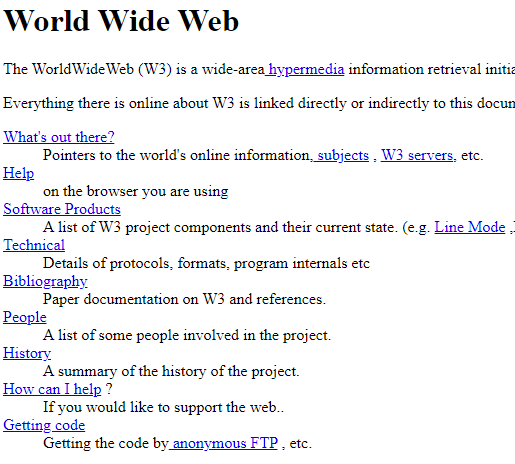
\includegraphics[width=12cm,keepaspectratio]{images/first_website.png}
	\caption{First Website [source: author]}
	\label{fig:first-website}
\end{figure}

\textbf{Web 2.0}\\
The term for the web 2.0 was first coined in 2004 by Dale Dougherty and Craig Cline in a conference with Tim O'Reilly. The key difference to the first iteration of the web, is that the second web allows read and write access instead of mostly read access. This could also be described as the first "dynamic" web, in contrast to the "static" web 1.0. Through "social-media" websites, "blogs", etc. users can generate content on a website, this leads to the terms "participative" web and "people-centric" web, for the web 2.0. \cite{hiremath2016}\\

Tim O'Reilly describes the web 2.0 as network with "rich user experiences", which are provided by websites from major corporations, such as the google search engine. One of the key components is AJAX, which is composed of several technologies, such as XHTML and CSS to represent the data on website, the Dosument Object Model, XML and XSLT, XMLHttpRequest for asynchronos data retrieval and JavaScript to bind everything together.\cite{oreilly2007}\\

Nowadays there are of course several other or newer technologies and further developments of the web 2.0, however the core-concepts remain roughly the same.\\

This chapter should provide a general understanding of the history of the web, as well as a demarcation of the web 2.0 to the web 3.0.
The next chapter will introduce several definitions, as well as new technologies of the web 3.0. \\


\section{Web 3.0}

\subsection{Definition}



\newpage
\chapter{Challenges of the Web 3.0}

\newpage
\chapter{Opportunities of the Web 3.0}

\newpage
\chapter{Related Work}

\newpage
\chapter{Conclusion}

\newpage
\chapter{Future work}

\newpage
\chapter{Summary}

\newpage

% --- Bibliography ------------------------------------------------------

%IEEE Citation [1]
%\bibliographystyle{IEEEtran}
%for alphanumeric citation eg.: [ABC19]
%\bibliographystyle{alpha}

% List references I definitely want in the bibliography,
% regardless of whether or not I cite them in the thesis.

\newpage
\addcontentsline{toc}{chapter}{Bibliography}
\printbibliography
\newpage

% --- List of Figures ----------------------------------------------------

\addcontentsline{toc}{chapter}{List of Figures}
\listoffigures


% --- List of Tables -----------------------------------------------------

\newpage
\addcontentsline{toc}{chapter}{List of Tables}
\listoftables

% --- Appendix A -----------------------------------------------------

\backmatter
\appendix
\begin{appendices}
\chapter{Appendix}

(Hier können Schaltpläne, Programme usw. eingefügt werden.)

\clearpage
\end{appendices}

\end{document}
